\section{Story}

\subsection{Synopsis}

Alexandria 51 was a thriving and technologically advanced city before a great war reduced it to a ghost town. You are one of the scavengers roaming in Alexandria’s 51 ruins trying to find the mysterious artifact which caused the rapid technological progress of the city. You finally reached the core building of the city and try to get inside it. A trap is activated, and an extreme bright light blinds you and your fellow criminals. For a few moments you can see the magical artifact, but now you are stuck inside the building and you have to find the artifact and get out.

\subsection{Complete story}

Within a world of science and technology, Alexandria 51 was the peak in terms of innovations and research. Alas, torn to pieces after a great war, only the rests of the buildings remain as witnesses for this sorrowful loss for humanity... except for greedy scavengers that still wander in what remains of the ghost town.\\
Legend has it that a secretive government was hiding the truth about its unprecedented technological advancement: a magical broom deeply hidden within a highly protected safehouse, located just near the outskirts of the city.\\
You are one of the scavengers roaming in these lands and together with your fellow criminal companions, you are finally able to find the legendary place. Everything around it is beyond repair, but something still stands, so it’s worth checking out: who knows if the wondrous artifact could still be hidden somewhere inside?\\
Finally, you are able to reach what appears to be the core of the building: a reinforced case, made of an extremely hard material is keeping something protected inside of it but you aren’t able to tell exactly what. Greed is tempting, so you all reach out for it and try to open the case: suddenly, you are all blinded by an extreme light. While your eyes recover, you catch a glimpse of a flying broom, surrounded by a mystic aura: “Is that what we were looking for?”\\
Suddenly the ground shakes, with sound of thunder the ancient traps built to keep the broom inside activated around the unaware scavengers.\\
Nonetheless, everyone looks blinded by greed, shoving and pushing everything in the attempt to reach the magical artifact. Are you going to be the one who catches it? Or will you perish in the crumbling ruins?\\

\subsection{Narrative devices}

The story will be told visually, using a cut-scene when registering into the game, before choosing your avatar class.

\subsection{Story Board}

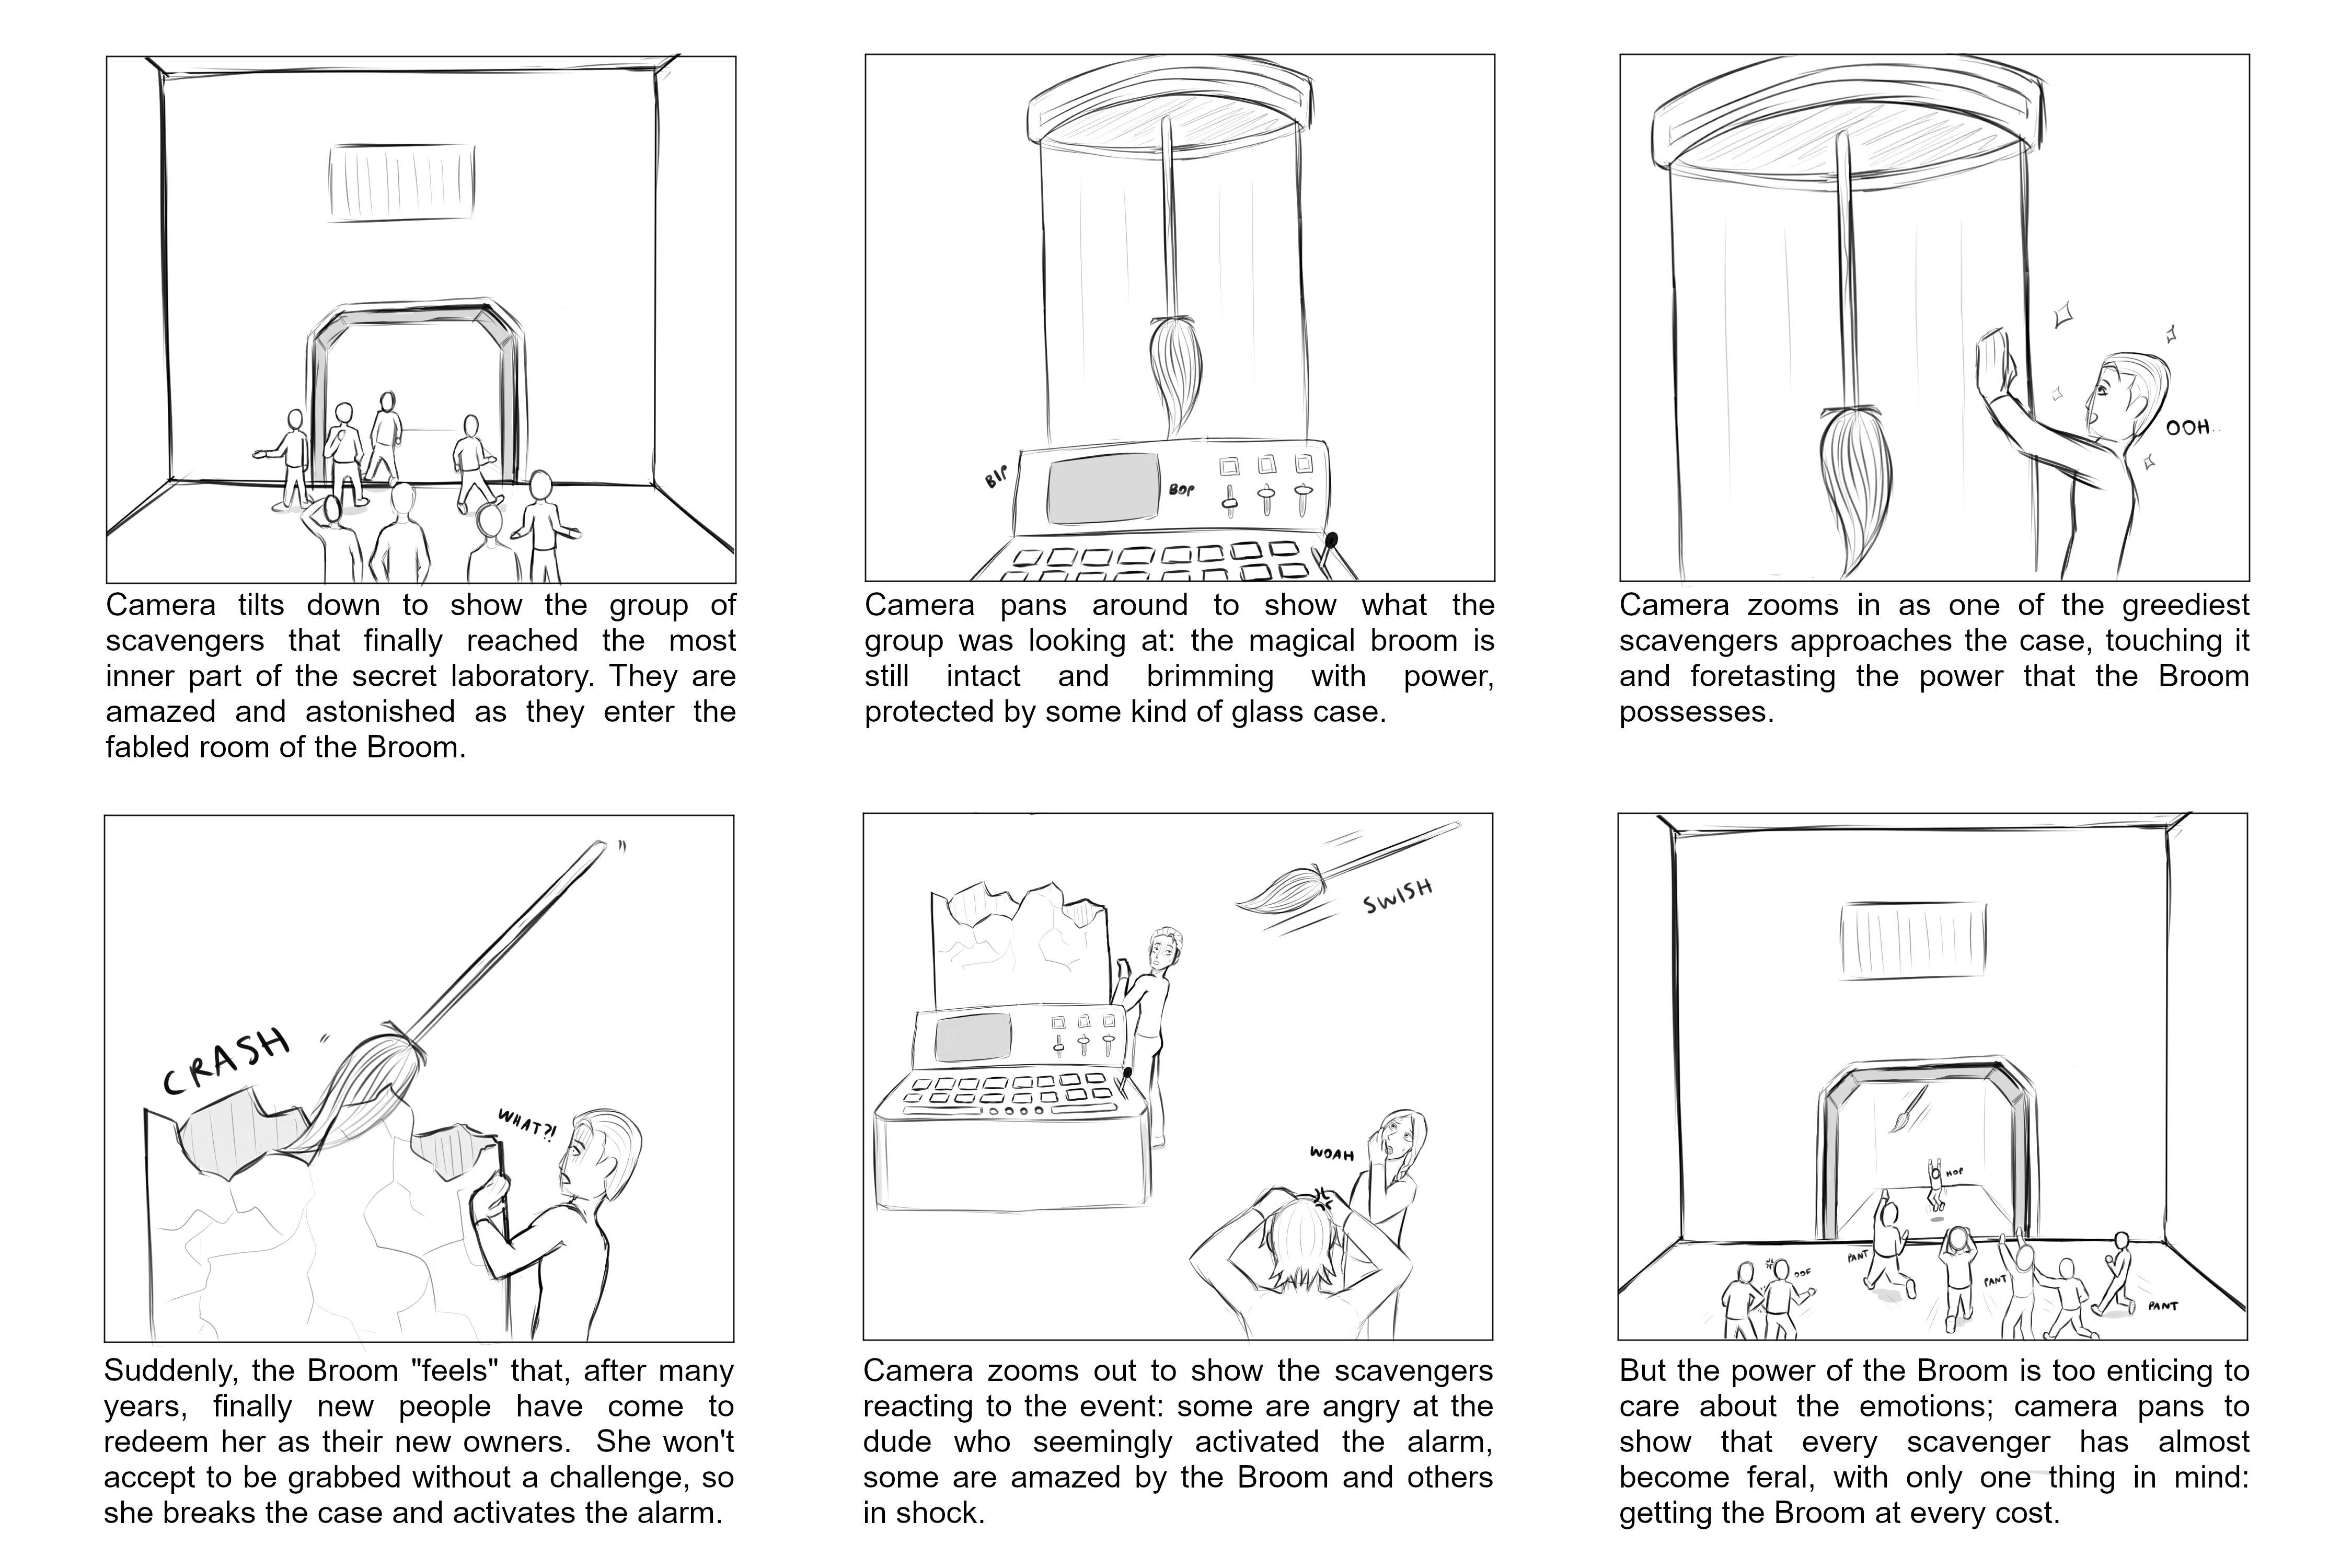
\includegraphics[height=\textwidth, angle=-90, origin=c]{../Pictures/Concept/Storyboard.png}
